\section{Iteración VII}
\subsection{Resumen}
Aquí desarrollamos una forma de gestionar escenarios dentro de la aplicación, mismos que son equivalentes a las propuestas de diseño de interiores.

\subsection{Desarrollo}
Una vez creado un proyecto, el usuario puede generar escenarios dentro de este, los cuales además de tener imagenes, tendrá la siguiente información general:
\begin{itemize}
	\item Nombre de escenario
	\item Tipo de habitación
	\item Tamaño de habitación
	\item Tipo de muebles
	\item Presupuesto del cliente
	\item Utilidad de la cotización
\end{itemize}

En la pantalla de visualización de proyecto, el usuario puede seleccionar la opción \textbf{ver escenarios} la cual mostrará en pantalla el listado de escenarios que hay en ese proyecto (ver figura x.xx). Cada escenario se muestra con una de las imagenes que contiene (ver figura x.xx). Al seleccionar un escenario se mostrarán las imagenes que lo conforman y al seleccionar una, se mostrará en pantalla completa (ver figura x.xx). De igual forma, el usuario podrá empezar a generar nuevos escenarios, siguiendo el siguiente proceso:
\begin{itemize}
	\item El usuario selecciona la opción para agregar un nuevo escenario al proyecto
	\item Se muestra un formulario con la información general del escenario, mismo que deberá ser llenado (ver figura x.xx).
	\item Cuando se llene el formulario, el usuario podrá acceder a la cámara para poder tomar las fotos que desee para conformar el escenario (ver figura x.xx). Dentro de la cámara el usuario podrá: agregar muebles a escena, cambiar de posición muebles agregados, eliminar muebles de escena, visualizar los precios de los muebles y tomar fotografías.
	\item Al finalizar el escenario, el usuario selecciona la opción \textbf{Guardar} y la aplicación mostrará una cuadrícula con las imágenes tomadas (ver figura x.xx).
	\item También habrá una opción \textbf{Ver cotización} misma que mostrará un subtotal con los precios de los muebles más la utilidad si es que se definió al crear el escenario, el IVA de este subtotal y la suma total de estos valores (ver figura x.xx).
\end{itemize}

Esta funcionalidad cumple tres procesos de negocios, correspondientes a las funciones de creación, lectura y actualización de escenarios (ver figuras x.xx, x.xx y x.xx)

\begin{figure}[h!]
	\centering
	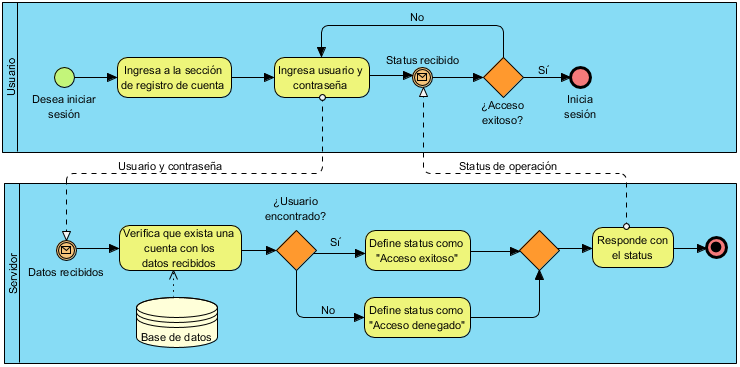
\includegraphics[width=15cm,height=9cm]{imagenes/desarrollo/diagramas/BPMN_LOGIN.png}
	\caption{Diagrama de proceso de recuperación de contraseña.}
	\label{fig:recover}
\end{figure}
\begin{figure}[h!]
	\centering
	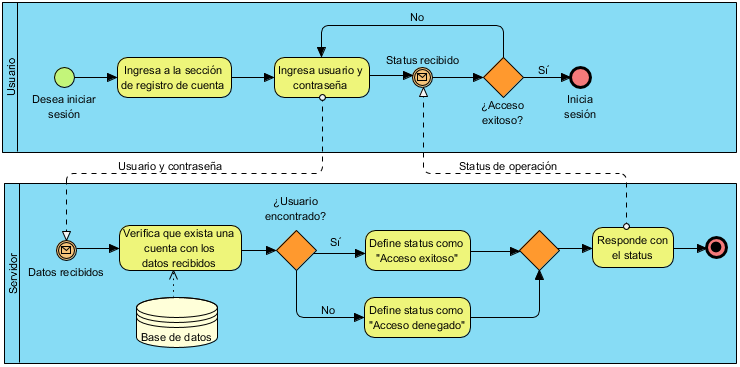
\includegraphics[width=15cm,height=9cm]{imagenes/desarrollo/diagramas/BPMN_LOGIN.png}
	\caption{Diagrama de proceso de recuperación de contraseña.}
	\label{fig:recover}
\end{figure}
\begin{figure}[h!]
	\centering
	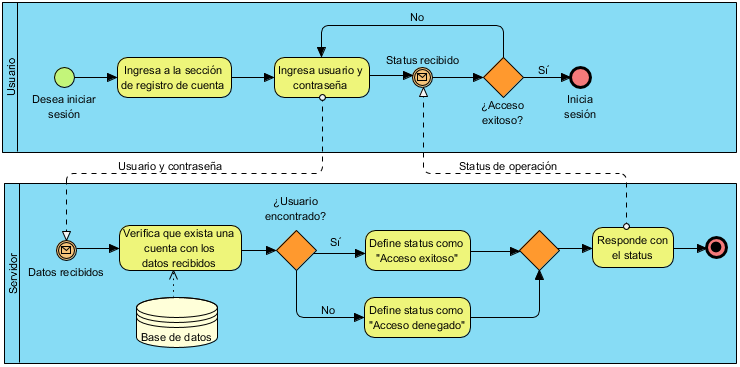
\includegraphics[width=15cm,height=9cm]{imagenes/desarrollo/diagramas/BPMN_LOGIN.png}
	\caption{Diagrama de proceso de recuperación de contraseña.}
	\label{fig:recover}
\end{figure}
\begin{figure}[h!]
	\centering
	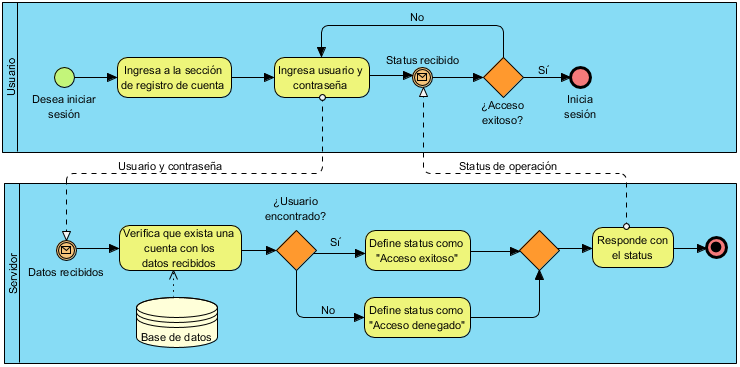
\includegraphics[width=15cm,height=9cm]{imagenes/desarrollo/diagramas/BPMN_LOGIN.png}
	\caption{Diagrama de proceso de recuperación de contraseña.}
	\label{fig:recover}
\end{figure}
\begin{figure}[h!]
	\centering
	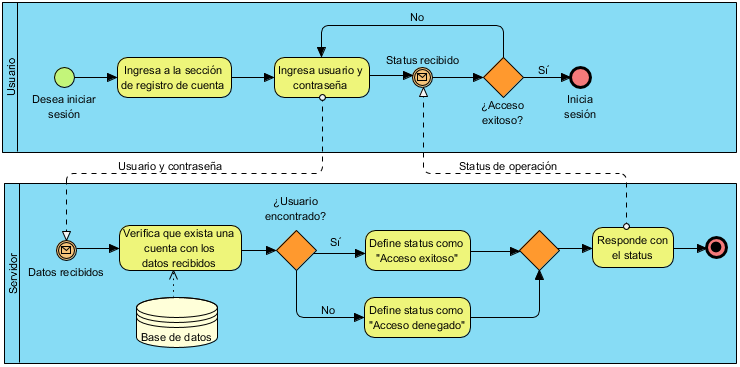
\includegraphics[width=15cm,height=9cm]{imagenes/desarrollo/diagramas/BPMN_LOGIN.png}
	\caption{Diagrama de proceso de recuperación de contraseña.}
	\label{fig:recover}
\end{figure}
\begin{figure}[h!]
	\centering
	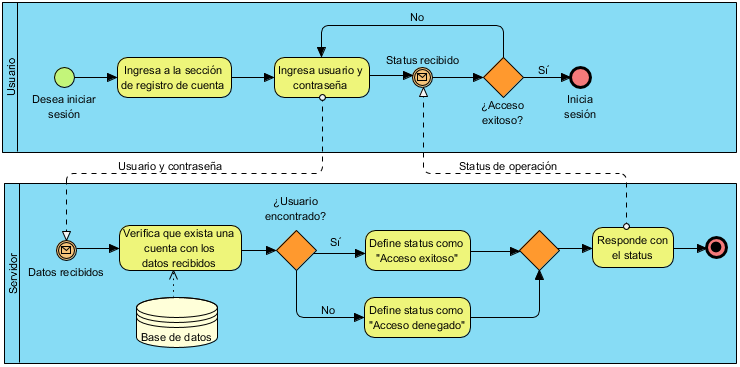
\includegraphics[width=15cm,height=9cm]{imagenes/desarrollo/diagramas/BPMN_LOGIN.png}
	\caption{Diagrama de proceso de recuperación de contraseña.}
	\label{fig:recover}
\end{figure}
\begin{figure}[h!]
	\centering
	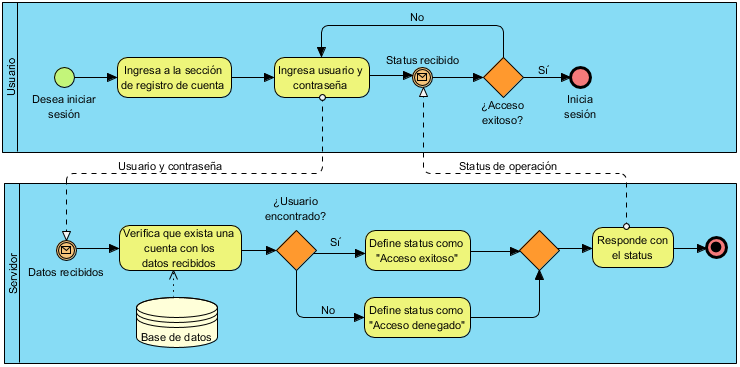
\includegraphics[width=15cm,height=9cm]{imagenes/desarrollo/diagramas/BPMN_LOGIN.png}
	\caption{Diagrama de proceso de recuperación de contraseña.}
	\label{fig:recover}
\end{figure}
